	\documentclass[twoside]{article}
\usepackage{../../estilo-ejercicios}

%--------------------------------------------------------
\begin{document}

\title{Relatión 1}
\author{Javier Aguilar Martín}
\maketitle


\begin{ejercicio}{1.1}

\end{ejercicio}
\begin{solucion}
Prueba que todo grafo bipartito de orden $n \geq 3$ es también $r$-partito para $3\leq r \leq n$. ¿Es
cierto el recíproco?
\end{solucion}

\newpage


\begin{ejercicio}{1.2}
Sea $T$ un árbol de orden $p$ que contiene $p_i$ vértices de grado $i$, para cada $i \in\{1,\dots, p-1\}$. Demuestra que $p_1 =
\sum^{p-1}_{i=3} (i - 2)p_i + 2$.
\end{ejercicio}
\begin{solucion}

\end{solucion}

\newpage

\begin{ejercicio}{1.3}

Sea $T$ un árbol de orden $p$ tal que todos sus vértices son de grado 1 o de grado 3. Prueba
que $T$ contiene exactamente $(p - 2)/2$ vértices de grado 3.
\end{ejercicio}
\begin{solucion}
\end{solucion}

\newpage

\begin{ejercicio}{1.4}

Encuentra todos los árboles $T$ tales que su complementario $\overline{T}$ es también un árbol.
\end{ejercicio}
\begin{solucion}

\end{solucion}

\newpage

\begin{ejercicio}{1.5}

Demuestra que todo árbol $T$ tiene un número de hojas mayor o igual que el grado máximo
de $T$.
\end{ejercicio}
\begin{solucion}

\end{solucion}

\newpage

\begin{ejercicio}{1.6}
Prueba que si $G$ es un grafo conexo de orden $p$ tal que todo subgrafo suyo de tamaño
$p -1$ es un árbol ``spanning'', entonces $G$ es un árbol o un ciclo.
\end{ejercicio}
\begin{solucion}
\end{solucion}

\newpage

\begin{ejercicio}{1.7}
Prueba o refuta el siguiente enunciado: Si $G$ es un grafo conexo tal que dos cualesquiera
de sus árboles ``spanning'' son isomorfos, entonces $G$ es un árbol o un ciclo.
\end{ejercicio}
\begin{solucion}

\end{solucion}

\newpage

\begin{ejercicio}{1.8}
Obtén un árbol spanning por el algoritmo DFS del grafo de Grotzsch de la figura adjunta.
\end{ejercicio}
\begin{solucion}





\end{solucion}
\newpage

\begin{ejercicio}{1.9}
Obtén un árbol spanning por el algoritmo DFS del grafo de Petersen de la figura adjunta.
\end{ejercicio}
\begin{solucion}

\end{solucion}
\newpage

\begin{ejercicio}{1.10}
Obtén un árbol spanning por el algoritmo DFS del grafo de Grotzsch de la figura adjunta.
\end{ejercicio}
\begin{solucion}

\end{solucion}

\newpage

\begin{ejercicio}{1.11}
Obtén un árbol spanning por el algoritmo BFS del grafo de Petersen de la figura adjunta.
\end{ejercicio}
\begin{solucion}



\end{solucion}

\newpage

\begin{figure}[h!]
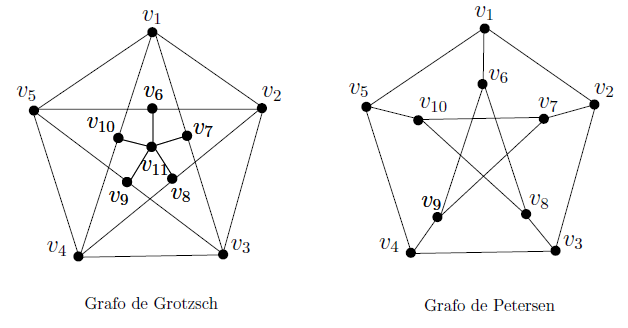
\includegraphics[scale=0.8]{Rel1}
\end{figure}
%
%\newpage
%
%\begin{ejercicio}{1.12}
%
%\end{ejercicio}
%\begin{solucion}
%
%\end{solucion}

\end{document}
